\chapter{目的} \label{cha:introduction}

\section{光生成反応\ref{fig:test1}}

宇宙線ミューオンが核子(陽子、中性子)と起こす反応に光生成反応がある。
この反応は核子とミューオンから出てくる光子との反応である。
また、この反応によりできるハドロン中間状態は、核子(N)と光子($\gamma$)の不変質量が小さい場合は短寿命の共鳴状態に近い。
また、終状態にはハドロンの中でも最も質量の小さいパイオン($\pi$)と陽子(p)の2つの粒子が出てくると期待される。

\begin{figure}[H]
	\centering
	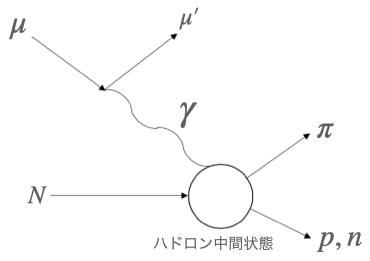
\includegraphics[width=10cm]{img/diagram_photoproduction.png}
	\caption{光生成反応のダイアグラム}
	\label{fig:test1}
\end{figure}

ハドロン中間状態の質量 $m_W$ は $\pi$ の質量$m_\pi$と陽子の質量 $m_p$の合計よりも大きくなければならない。

\begin{equation}
    m_W \geq m_\pi + m_p \approx 0.14 + 0.94 = 1.08 \ GeV
\end{equation}

次に三元運動量を考える。
核子、光子の三元運動量をそれぞれ$p_N$, $p_\gamma$とすると、\ref{fig:test1}

\begin{equation}
    p_N = (0, m_N),\  p_\gamma = (E_\gamma, E_\gamma)
\end{equation}
とかけ、$m_W$との関係は

\begin{equation}
    m_W^2 = (p_N + p_\gamma)^2 = p_N^2 + 2p_N p_\gamma + p_\gamma^2
          = 2m_N E_\gamma + m_N^2 
\end{equation}
(1.3)式から$m_W$ = 1.08 GeV の時、$m_N$ = 0.94 GeVであるから

\begin{figure}[H]
	\centering
	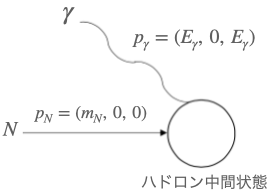
\includegraphics[width=10cm]{img/diagram_momentum.png}
	\caption{ハドロン中間状態と核子と光子の図}
	\label{fig:test2}
\end{figure}

\begin{equation}
    E_\gamma \approx 0.23 GeV
\end{equation}

よって、光生成反応を観測するために必要な光子のエネルギー$E_\gamma$は
$E_\gamma \geq 0.23 GeV$となる。